\documentclass[a4paper,11pt,dvipdfmx]{ujarticle}
% パッケージ
\usepackage{graphicx}
\usepackage{url}
% レイアウト指定を記述したファイルの読み込み
\input{layout}

% タイトルと氏名を変更せよ.
\title{日本におけるデジタル化の状況}
\author{G585052025渡辺 恒之介}

\begin{document}

\maketitle %ここにタイトルが入る

% ここから本文
% 節見出し: \section{}
% を使う
\section{デジタル競争力ランキング}

% 本文(1)
%  参考文献の参照: \cite{}
%  図番号の参照: \ref{}
% を使う
% 文献データベースのキーワードは oecd と imd
% になっている.
国際経営開発研究所(IMD)の調査\cite{imd}によると、
日本のデジタル競争力のランキングは図\ref{zu}に示すように、
調査対象の64カ国中、総合で28位。知識分野で25位となっている。

% 図の挿入
% \includegraphics{}
% を
% \begin{figure}[htbp]
% \end{figure}
% で囲み
% \caption{}
% で図のタイトルを入れる.
% \label{}
% を使って図番号が参照できるようにする
% また,
% \centering
% で図が中央に来るようにする
\begin{figure}[htbp]
    \label{zu}
    \centering
    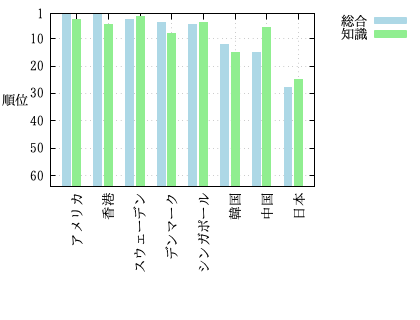
\includegraphics{fig31.png}
    \caption{デジタル競争力ランキング (64カ国中)}
\end{figure}

% ーーー
% 節見出し(2)
\section{ブロードバンドの整備状況}
% 本文(2)

OECDによるブロードバンド回線の普及に関する調査\cite{oecd}によると、
表\ref{hyou}に示すように、日本における100人あたりの光ファイバー回線の
加入者数は29.0で,韓国、スウェーデン、ノルウェーに続いて第
4位になっている。
% 表の挿入
% \begin{tabular}
% \end{tabular}    
% による表の記述を 
% \begin{table}[htbp]
% \end{table}
% で囲み
% \caption{}
% で表のタイトルを入れる.
% \label{}
% を使って表番号が参照できるようにする
% また,
% \centering
% で表が中央に来るようにする

\begin{table}[htbp]
    \centering
    \caption{光ファイバー回線の加入者数(100人あたり)}
    \label{hyou}

    \begin{tabular}{|c|l|r|}\hline
        順位 & 国名 & 加入者数 \\
        \hline
        1位 & 韓国 & 38.2 \\
        \hline
        2位 & スウェーデン & 31.9 \\
        \hline
        3位 & ノルウェー & 29.5 \\
        \hline
        4位 & 日本 & 29.0 \\
        \hline
        5位 & アイスランド & 28.8 \\
        \hline
        6位 & スペイン & 27.3 \\
        \hline
        7位 & ポルトガル & 25.1 \\
        \hline
        8位 & ニュージーランド & 23.6 \\
        \hline
        9位 & リトアニア & 22.3 \\
        \hline
        10位 & フランス & 21.2 \\
        \hline
        
    \end{tabular}
\end{table}
% ーーー
% 見出し(3)
\section{考察}
% 考察
%
% \begin{itemize}
% \end{itemize}
% を使って箇条書きで記述する
\begin{itemize}
    \item 日本のデジタル競争力ランキングについて
    \begin{itemize}
    \item 総合28位、知識分野で25位とかなり低い
    \item 知識分野よりも総合が低いのは、技術力などが知識に追いついていないのではないかと感じた
    \end{itemize}
    \item 日本の光ファイバーの加入者数について
    \begin{itemize}
    \item 世界4位、約3割が加入とかなり高い
    \end{itemize}
    \item 2つの統計を比較して
    \begin{itemize}
    \item 2つの統計に相関関係がないことが分かった
    \item 2つの統計の順位差は、一般人への普及をどれだけ意識しているかが関わっているのではないかと感じた
    \end{itemize}
\end{itemize}
% ここに参考文献が入る
%
\bibliographystyle{junsrt}
\bibliography{exercise.bib}

\end{document}